% Options for packages loaded elsewhere
\PassOptionsToPackage{unicode}{hyperref}
\PassOptionsToPackage{hyphens}{url}
\PassOptionsToPackage{dvipsnames,svgnames,x11names}{xcolor}
%
\documentclass[
  letterpaper,
  DIV=11,
  numbers=noendperiod]{scrartcl}

\usepackage{amsmath,amssymb}
\usepackage{lmodern}
\usepackage{iftex}
\ifPDFTeX
  \usepackage[T1]{fontenc}
  \usepackage[utf8]{inputenc}
  \usepackage{textcomp} % provide euro and other symbols
\else % if luatex or xetex
  \usepackage{unicode-math}
  \defaultfontfeatures{Scale=MatchLowercase}
  \defaultfontfeatures[\rmfamily]{Ligatures=TeX,Scale=1}
\fi
% Use upquote if available, for straight quotes in verbatim environments
\IfFileExists{upquote.sty}{\usepackage{upquote}}{}
\IfFileExists{microtype.sty}{% use microtype if available
  \usepackage[]{microtype}
  \UseMicrotypeSet[protrusion]{basicmath} % disable protrusion for tt fonts
}{}
\makeatletter
\@ifundefined{KOMAClassName}{% if non-KOMA class
  \IfFileExists{parskip.sty}{%
    \usepackage{parskip}
  }{% else
    \setlength{\parindent}{0pt}
    \setlength{\parskip}{6pt plus 2pt minus 1pt}}
}{% if KOMA class
  \KOMAoptions{parskip=half}}
\makeatother
\usepackage{xcolor}
\setlength{\emergencystretch}{3em} % prevent overfull lines
\setcounter{secnumdepth}{-\maxdimen} % remove section numbering
% Make \paragraph and \subparagraph free-standing
\ifx\paragraph\undefined\else
  \let\oldparagraph\paragraph
  \renewcommand{\paragraph}[1]{\oldparagraph{#1}\mbox{}}
\fi
\ifx\subparagraph\undefined\else
  \let\oldsubparagraph\subparagraph
  \renewcommand{\subparagraph}[1]{\oldsubparagraph{#1}\mbox{}}
\fi

\usepackage{color}
\usepackage{fancyvrb}
\newcommand{\VerbBar}{|}
\newcommand{\VERB}{\Verb[commandchars=\\\{\}]}
\DefineVerbatimEnvironment{Highlighting}{Verbatim}{commandchars=\\\{\}}
% Add ',fontsize=\small' for more characters per line
\usepackage{framed}
\definecolor{shadecolor}{RGB}{241,243,245}
\newenvironment{Shaded}{\begin{snugshade}}{\end{snugshade}}
\newcommand{\AlertTok}[1]{\textcolor[rgb]{0.68,0.00,0.00}{#1}}
\newcommand{\AnnotationTok}[1]{\textcolor[rgb]{0.37,0.37,0.37}{#1}}
\newcommand{\AttributeTok}[1]{\textcolor[rgb]{0.40,0.45,0.13}{#1}}
\newcommand{\BaseNTok}[1]{\textcolor[rgb]{0.68,0.00,0.00}{#1}}
\newcommand{\BuiltInTok}[1]{\textcolor[rgb]{0.00,0.23,0.31}{#1}}
\newcommand{\CharTok}[1]{\textcolor[rgb]{0.13,0.47,0.30}{#1}}
\newcommand{\CommentTok}[1]{\textcolor[rgb]{0.37,0.37,0.37}{#1}}
\newcommand{\CommentVarTok}[1]{\textcolor[rgb]{0.37,0.37,0.37}{\textit{#1}}}
\newcommand{\ConstantTok}[1]{\textcolor[rgb]{0.56,0.35,0.01}{#1}}
\newcommand{\ControlFlowTok}[1]{\textcolor[rgb]{0.00,0.23,0.31}{#1}}
\newcommand{\DataTypeTok}[1]{\textcolor[rgb]{0.68,0.00,0.00}{#1}}
\newcommand{\DecValTok}[1]{\textcolor[rgb]{0.68,0.00,0.00}{#1}}
\newcommand{\DocumentationTok}[1]{\textcolor[rgb]{0.37,0.37,0.37}{\textit{#1}}}
\newcommand{\ErrorTok}[1]{\textcolor[rgb]{0.68,0.00,0.00}{#1}}
\newcommand{\ExtensionTok}[1]{\textcolor[rgb]{0.00,0.23,0.31}{#1}}
\newcommand{\FloatTok}[1]{\textcolor[rgb]{0.68,0.00,0.00}{#1}}
\newcommand{\FunctionTok}[1]{\textcolor[rgb]{0.28,0.35,0.67}{#1}}
\newcommand{\ImportTok}[1]{\textcolor[rgb]{0.00,0.46,0.62}{#1}}
\newcommand{\InformationTok}[1]{\textcolor[rgb]{0.37,0.37,0.37}{#1}}
\newcommand{\KeywordTok}[1]{\textcolor[rgb]{0.00,0.23,0.31}{#1}}
\newcommand{\NormalTok}[1]{\textcolor[rgb]{0.00,0.23,0.31}{#1}}
\newcommand{\OperatorTok}[1]{\textcolor[rgb]{0.37,0.37,0.37}{#1}}
\newcommand{\OtherTok}[1]{\textcolor[rgb]{0.00,0.23,0.31}{#1}}
\newcommand{\PreprocessorTok}[1]{\textcolor[rgb]{0.68,0.00,0.00}{#1}}
\newcommand{\RegionMarkerTok}[1]{\textcolor[rgb]{0.00,0.23,0.31}{#1}}
\newcommand{\SpecialCharTok}[1]{\textcolor[rgb]{0.37,0.37,0.37}{#1}}
\newcommand{\SpecialStringTok}[1]{\textcolor[rgb]{0.13,0.47,0.30}{#1}}
\newcommand{\StringTok}[1]{\textcolor[rgb]{0.13,0.47,0.30}{#1}}
\newcommand{\VariableTok}[1]{\textcolor[rgb]{0.07,0.07,0.07}{#1}}
\newcommand{\VerbatimStringTok}[1]{\textcolor[rgb]{0.13,0.47,0.30}{#1}}
\newcommand{\WarningTok}[1]{\textcolor[rgb]{0.37,0.37,0.37}{\textit{#1}}}

\providecommand{\tightlist}{%
  \setlength{\itemsep}{0pt}\setlength{\parskip}{0pt}}\usepackage{longtable,booktabs,array}
\usepackage{calc} % for calculating minipage widths
% Correct order of tables after \paragraph or \subparagraph
\usepackage{etoolbox}
\makeatletter
\patchcmd\longtable{\par}{\if@noskipsec\mbox{}\fi\par}{}{}
\makeatother
% Allow footnotes in longtable head/foot
\IfFileExists{footnotehyper.sty}{\usepackage{footnotehyper}}{\usepackage{footnote}}
\makesavenoteenv{longtable}
\usepackage{graphicx}
\makeatletter
\def\maxwidth{\ifdim\Gin@nat@width>\linewidth\linewidth\else\Gin@nat@width\fi}
\def\maxheight{\ifdim\Gin@nat@height>\textheight\textheight\else\Gin@nat@height\fi}
\makeatother
% Scale images if necessary, so that they will not overflow the page
% margins by default, and it is still possible to overwrite the defaults
% using explicit options in \includegraphics[width, height, ...]{}
\setkeys{Gin}{width=\maxwidth,height=\maxheight,keepaspectratio}
% Set default figure placement to htbp
\makeatletter
\def\fps@figure{htbp}
\makeatother
\newlength{\cslhangindent}
\setlength{\cslhangindent}{1.5em}
\newlength{\csllabelwidth}
\setlength{\csllabelwidth}{3em}
\newlength{\cslentryspacingunit} % times entry-spacing
\setlength{\cslentryspacingunit}{\parskip}
\newenvironment{CSLReferences}[2] % #1 hanging-ident, #2 entry spacing
 {% don't indent paragraphs
  \setlength{\parindent}{0pt}
  % turn on hanging indent if param 1 is 1
  \ifodd #1
  \let\oldpar\par
  \def\par{\hangindent=\cslhangindent\oldpar}
  \fi
  % set entry spacing
  \setlength{\parskip}{#2\cslentryspacingunit}
 }%
 {}
\usepackage{calc}
\newcommand{\CSLBlock}[1]{#1\hfill\break}
\newcommand{\CSLLeftMargin}[1]{\parbox[t]{\csllabelwidth}{#1}}
\newcommand{\CSLRightInline}[1]{\parbox[t]{\linewidth - \csllabelwidth}{#1}\break}
\newcommand{\CSLIndent}[1]{\hspace{\cslhangindent}#1}

\usepackage{amsmath}
\usepackage{booktabs}
\usepackage{caption}
\usepackage{longtable}
\KOMAoption{captions}{tableheading}
\makeatletter
\makeatother
\makeatletter
\makeatother
\makeatletter
\@ifpackageloaded{caption}{}{\usepackage{caption}}
\AtBeginDocument{%
\ifdefined\contentsname
  \renewcommand*\contentsname{Índice}
\else
  \newcommand\contentsname{Índice}
\fi
\ifdefined\listfigurename
  \renewcommand*\listfigurename{Lista de Figuras}
\else
  \newcommand\listfigurename{Lista de Figuras}
\fi
\ifdefined\listtablename
  \renewcommand*\listtablename{Lista de Tabelas}
\else
  \newcommand\listtablename{Lista de Tabelas}
\fi
\ifdefined\figurename
  \renewcommand*\figurename{Figura}
\else
  \newcommand\figurename{Figura}
\fi
\ifdefined\tablename
  \renewcommand*\tablename{Tabela}
\else
  \newcommand\tablename{Tabela}
\fi
}
\@ifpackageloaded{float}{}{\usepackage{float}}
\floatstyle{ruled}
\@ifundefined{c@chapter}{\newfloat{codelisting}{h}{lop}}{\newfloat{codelisting}{h}{lop}[chapter]}
\floatname{codelisting}{Listagem}
\newcommand*\listoflistings{\listof{codelisting}{Lista de Listagens}}
\makeatother
\makeatletter
\@ifpackageloaded{caption}{}{\usepackage{caption}}
\@ifpackageloaded{subcaption}{}{\usepackage{subcaption}}
\makeatother
\makeatletter
\@ifpackageloaded{tcolorbox}{}{\usepackage[many]{tcolorbox}}
\makeatother
\makeatletter
\@ifundefined{shadecolor}{\definecolor{shadecolor}{rgb}{.97, .97, .97}}
\makeatother
\makeatletter
\makeatother
\ifLuaTeX
\usepackage[bidi=basic]{babel}
\else
\usepackage[bidi=default]{babel}
\fi
\babelprovide[main,import]{portuguese}
% get rid of language-specific shorthands (see #6817):
\let\LanguageShortHands\languageshorthands
\def\languageshorthands#1{}
\ifLuaTeX
  \usepackage{selnolig}  % disable illegal ligatures
\fi
\IfFileExists{bookmark.sty}{\usepackage{bookmark}}{\usepackage{hyperref}}
\IfFileExists{xurl.sty}{\usepackage{xurl}}{} % add URL line breaks if available
\urlstyle{same} % disable monospaced font for URLs
\hypersetup{
  pdftitle={Informações sobre barragens de mineração},
  pdfauthor={Márcio Augusto F. Rodrigues},
  pdflang={pt},
  colorlinks=true,
  linkcolor={blue},
  filecolor={Maroon},
  citecolor={Blue},
  urlcolor={Blue},
  pdfcreator={LaTeX via pandoc}}

\title{Informações sobre barragens de mineração}
\author{Márcio Augusto F. Rodrigues}
\date{Agosto de 2022}

\begin{document}
\maketitle
\ifdefined\Shaded\renewenvironment{Shaded}{\begin{tcolorbox}[boxrule=0pt, breakable, sharp corners, frame hidden, borderline west={3pt}{0pt}{shadecolor}, interior hidden, enhanced]}{\end{tcolorbox}}\fi

\hypertarget{sec-objetivos}{%
\subsection{Objetivos}\label{sec-objetivos}}

Este relatório tem como objetivo apresentar funcionalidades do \emph{R
Markdown} e do \emph{Quarto}, utilizando dados públicos sobre barragens
de mineração no Brasil.

Os objetivos específicos da análise são:

\begin{itemize}
\tightlist
\item
  fazer uma tabela das barragens por estado;
\item
  fazer um gráfico do número de barragens por categoria de dano
  potencial associado;
\end{itemize}

\hypertarget{materiais-e-muxe9todos}{%
\subsection{Materiais e métodos}\label{materiais-e-muxe9todos}}

A base de dados disponibilizada pelo
\href{https://app.anm.gov.br/SIGBM/Publico/ClassificacaoNacionalDaBarragem}{SIGBM
- Sistema de Gestão de Segurança de Barragem de Mineração} apresenta
dados referentes à Barragens de Mineração no território brasileiro.


\includegraphics{https://app.anm.gov.br/SIGBM/Content/images/anm315x66azul_r.png}

\hypertarget{carregando-os-pacotes}{%
\subsection{Carregando os pacotes}\label{carregando-os-pacotes}}

\begin{Shaded}
\begin{Highlighting}[]
\FunctionTok{library}\NormalTok{(gt)}
\FunctionTok{library}\NormalTok{(janitor)}
\FunctionTok{library}\NormalTok{(tidyverse)}
\FunctionTok{library}\NormalTok{(readxl)}
\end{Highlighting}
\end{Shaded}

\hypertarget{download-e-leitura-da-base}{%
\subsection{Download e leitura da
base}\label{download-e-leitura-da-base}}

\hypertarget{download}{%
\subsubsection{Download}\label{download}}

\hypertarget{leitura}{%
\subsubsection{Leitura}\label{leitura}}

\begin{Shaded}
\begin{Highlighting}[]
\CommentTok{\# Importar a base de dados:}
\CommentTok{\# ler os dados baixados}
\NormalTok{sigbm }\OtherTok{\textless{}{-}} \FunctionTok{read\_xlsx}\NormalTok{(}\StringTok{"dados/sigbm.xlsx"}\NormalTok{, }\AttributeTok{skip =} \DecValTok{4}\NormalTok{) }\SpecialCharTok{|\textgreater{}}
  \FunctionTok{clean\_names}\NormalTok{()}
\end{Highlighting}
\end{Shaded}

Data de atualização da base

\begin{Shaded}
\begin{Highlighting}[]
\CommentTok{\# {-}{-}{-}{-}{-} data de atualização {-}{-}{-}{-}{-}}
\NormalTok{data\_atualizacao\_sigbm }\OtherTok{\textless{}{-}} \FunctionTok{read\_xlsx}\NormalTok{(}\StringTok{"dados/sigbm.xlsx"}\NormalTok{,}
                                    \AttributeTok{col\_names =} \ConstantTok{FALSE}\NormalTok{,}
                                    \AttributeTok{n\_max =} \DecValTok{1}\NormalTok{) }\SpecialCharTok{|\textgreater{}}
  \FunctionTok{pull}\NormalTok{() }\SpecialCharTok{|\textgreater{}}
  \FunctionTok{str\_extract}\NormalTok{(}\StringTok{":.*{-}"}\NormalTok{) }\SpecialCharTok{|\textgreater{}}
  \FunctionTok{str\_remove}\NormalTok{(}\StringTok{":"}\NormalTok{) }\SpecialCharTok{|\textgreater{}}
  \FunctionTok{str\_remove}\NormalTok{(}\StringTok{"{-}"}\NormalTok{) }\SpecialCharTok{|\textgreater{}}
  \FunctionTok{str\_trim}\NormalTok{()}
\end{Highlighting}
\end{Shaded}

\hypertarget{barragens-de-minerauxe7uxe3o-no-brasil}{%
\subsection{Barragens de mineração no
Brasil}\label{barragens-de-minerauxe7uxe3o-no-brasil}}

A base do SIGBM foi obtida no dia 30/08/2022, e apresentou informações
referentes a 912.

\hypertarget{tabela}{%
\subsection{Tabela}\label{tabela}}

\begin{Shaded}
\begin{Highlighting}[]
\NormalTok{sigbm }\SpecialCharTok{|\textgreater{}}
  \FunctionTok{count}\NormalTok{(uf, }\AttributeTok{sort =} \ConstantTok{TRUE}\NormalTok{) }\SpecialCharTok{|\textgreater{}}
  \FunctionTok{slice}\NormalTok{(}\DecValTok{1}\SpecialCharTok{:}\DecValTok{10}\NormalTok{) }\SpecialCharTok{|\textgreater{}}
  \FunctionTok{select}\NormalTok{(}\StringTok{\textasciigrave{}}\AttributeTok{Estado}\StringTok{\textasciigrave{}} \OtherTok{=}\NormalTok{ uf, }\StringTok{\textasciigrave{}}\AttributeTok{Número de barragens}\StringTok{\textasciigrave{}} \OtherTok{=}\NormalTok{ n) }\SpecialCharTok{|\textgreater{}}
\NormalTok{  gt}\SpecialCharTok{::}\FunctionTok{gt}\NormalTok{(}\AttributeTok{caption =} \StringTok{"Dez estados brasileiros com mais barragens cadastradas no SIG{-}BM"}\NormalTok{)}
\end{Highlighting}
\end{Shaded}

\captionsetup[table]{labelformat=empty,skip=1pt}
\begin{longtable}{lr}
\toprule
Estado & Número de barragens \\ 
\midrule
MG & 347 \\ 
MT & 152 \\ 
PA & 114 \\ 
BA & 82 \\ 
SP & 68 \\ 
RO & 36 \\ 
GO & 22 \\ 
AP & 18 \\ 
MS & 18 \\ 
AM & 15 \\ 
\bottomrule
\end{longtable}

\hypertarget{gruxe1fico}{%
\subsection{Gráfico}\label{gruxe1fico}}

\begin{Shaded}
\begin{Highlighting}[]
\DocumentationTok{\#\# {-}{-}{-}{-}plot{-}dpa{-}{-}{-}{-}{-}{-}{-}{-}{-}{-}{-}{-}{-}{-}{-}{-}{-}{-}{-}{-}{-}{-}{-}{-}{-}{-}{-}}
\NormalTok{sigbm }\SpecialCharTok{|\textgreater{}}
  \FunctionTok{count}\NormalTok{(dano\_potencial\_associado) }\SpecialCharTok{|\textgreater{}}
    \FunctionTok{mutate}\NormalTok{(}
    \AttributeTok{dano\_potencial\_associado =} \FunctionTok{if\_else}\NormalTok{(}
\NormalTok{      dano\_potencial\_associado }\SpecialCharTok{==} \StringTok{"N/A"}\NormalTok{,}
      \StringTok{"Não se aplica"}\NormalTok{,}
\NormalTok{      dano\_potencial\_associado}
\NormalTok{    ),}
    \AttributeTok{dano\_potencial\_associado =} \FunctionTok{factor}\NormalTok{(}
\NormalTok{      dano\_potencial\_associado,}
      \AttributeTok{levels =} \FunctionTok{c}\NormalTok{(}\StringTok{"Não se aplica"}\NormalTok{, }\StringTok{"Baixo"}\NormalTok{, }\StringTok{"Médio"}\NormalTok{, }\StringTok{"Alto"}\NormalTok{)}
\NormalTok{    )}
\NormalTok{  ) }\SpecialCharTok{|\textgreater{}}
  \FunctionTok{ggplot}\NormalTok{() }\SpecialCharTok{+}
  \FunctionTok{aes}\NormalTok{(}\AttributeTok{x =}\NormalTok{ dano\_potencial\_associado, }\AttributeTok{y =}\NormalTok{ n) }\SpecialCharTok{+}
  \FunctionTok{geom\_col}\NormalTok{(}\AttributeTok{fill =} \StringTok{"lightblue"}\NormalTok{) }\SpecialCharTok{+}
  \FunctionTok{theme\_bw}\NormalTok{() }\SpecialCharTok{+}
  \FunctionTok{labs}\NormalTok{(}\AttributeTok{x =} \StringTok{"Dano potencial associado (DPA)"}\NormalTok{, }\AttributeTok{y =} \StringTok{"Quantidade de barragens"}\NormalTok{,}
       \AttributeTok{title =} \StringTok{"Dano potencial associado de barragens de mineração no Brasil"}\NormalTok{)}
\end{Highlighting}
\end{Shaded}

\begin{figure}[H]

{\centering 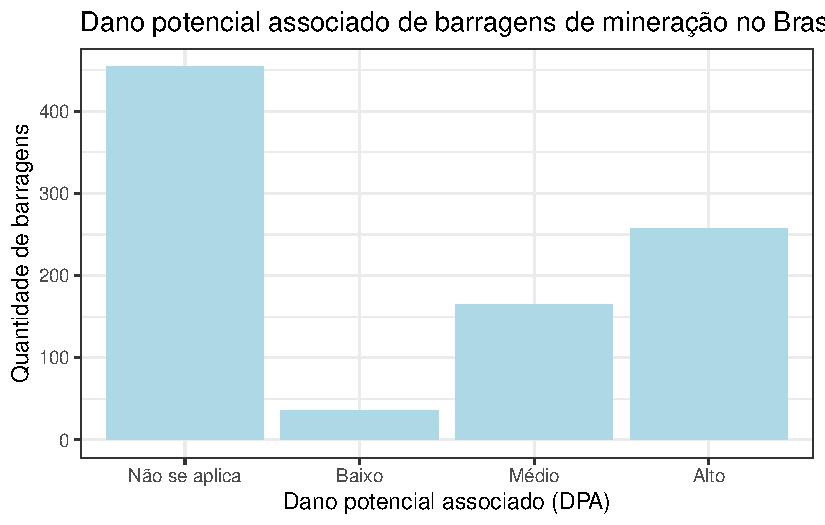
\includegraphics[width=0.95\textwidth,height=\textheight]{pratica3_files/figure-pdf/fig-grafico-dpa-1.pdf}

}

\caption{\label{fig-grafico-dpa}Gráfico do número de barragens segundo o
Dano Potencial Associado}

\end{figure}

\hypertarget{aula-2}{%
\subsection{Aula 2}\label{aula-2}}

\begin{Shaded}
\begin{Highlighting}[]
\NormalTok{knitr}\SpecialCharTok{::}\FunctionTok{include\_graphics}\NormalTok{(}\StringTok{"https://www.r{-}project.org/Rlogo.png"}\NormalTok{)}
\end{Highlighting}
\end{Shaded}

\begin{figure}[H]

\hfill{} \includegraphics[width=0.1\textwidth,height=\textheight]{https://www.r-project.org/Rlogo.png}

\caption{Logo do R}

\end{figure}

\hypertarget{tabelas}{%
\subsubsection{Tabelas}\label{tabelas}}

\begin{Shaded}
\begin{Highlighting}[]
\NormalTok{top10uf }\OtherTok{\textless{}{-}}\NormalTok{ sigbm }\SpecialCharTok{|\textgreater{}}
  \FunctionTok{count}\NormalTok{(uf, }\AttributeTok{sort =} \ConstantTok{TRUE}\NormalTok{) }\SpecialCharTok{|\textgreater{}}
  \FunctionTok{slice}\NormalTok{(}\DecValTok{1}\SpecialCharTok{:}\DecValTok{10}\NormalTok{) }\SpecialCharTok{|\textgreater{}}
  \FunctionTok{select}\NormalTok{(}\StringTok{\textasciigrave{}}\AttributeTok{Estado}\StringTok{\textasciigrave{}} \OtherTok{=}\NormalTok{ uf, }\StringTok{\textasciigrave{}}\AttributeTok{Número de barragens}\StringTok{\textasciigrave{}} \OtherTok{=}\NormalTok{ n)}
\end{Highlighting}
\end{Shaded}

\begin{itemize}
\tightlist
\item
  Com knitr:
\end{itemize}

\begin{Shaded}
\begin{Highlighting}[]
\NormalTok{top10uf }\SpecialCharTok{|\textgreater{}} 
\NormalTok{  knitr}\SpecialCharTok{::}\FunctionTok{kable}\NormalTok{()}
\end{Highlighting}
\end{Shaded}

\begin{longtable}[]{@{}lr@{}}
\toprule()
Estado & Número de barragens \\
\midrule()
\endhead
MG & 347 \\
MT & 152 \\
PA & 114 \\
BA & 82 \\
SP & 68 \\
RO & 36 \\
GO & 22 \\
AP & 18 \\
MS & 18 \\
AM & 15 \\
\bottomrule()
\end{longtable}

\begin{itemize}
\tightlist
\item
  Com gt:
\end{itemize}

\begin{Shaded}
\begin{Highlighting}[]
\CommentTok{\# top10uf |\textgreater{} }
\CommentTok{\#   gt::gt()}
\end{Highlighting}
\end{Shaded}

\begin{itemize}
\tightlist
\item
  Com DT:
\end{itemize}

\begin{Shaded}
\begin{Highlighting}[]
\CommentTok{\# top10uf |\textgreater{} }
\CommentTok{\#   DT::datatable()}
\end{Highlighting}
\end{Shaded}

\begin{itemize}
\tightlist
\item
  Com reactable:
\end{itemize}

\begin{Shaded}
\begin{Highlighting}[]
\CommentTok{\# top10uf |\textgreater{} }
\CommentTok{\#   reactable::reactable()}
\end{Highlighting}
\end{Shaded}

\begin{itemize}
\tightlist
\item
  Com flextable:
\end{itemize}

\begin{Shaded}
\begin{Highlighting}[]
\CommentTok{\# top10uf |\textgreater{} }
\CommentTok{\#   flextable::flextable()}
\end{Highlighting}
\end{Shaded}

\hypertarget{cuxf3digo-inline}{%
\subsubsection{Código inline}\label{cuxf3digo-inline}}

A base mtcars possui 32 carros. As colunas presentes na base são mpg,
cyl, disp, hp, drat, wt, qsec, vs, am, gear, e carb.

\hypertarget{equauxe7uxf5es-com-latex}{%
\subsubsection{Equações com Latex}\label{equauxe7uxf5es-com-latex}}

A equação da média é
\({\text{Média}=\frac {a_{1}+a_{2}+\cdots +a_{n}}{n}}\), sendo usada
amplamente para análises descritivas.

\[{\text{Média}=\frac {a_{1}+a_{2}+\cdots +a_{n}}{n}}\]

\hypertarget{adicionar-referuxeancias}{%
\subsubsection{Adicionar referências}\label{adicionar-referuxeancias}}

Outros estudos utilizaram dados do SIGBM, como LEÃO; SANTIAGO (2022)

Esse relatório foi feito usando R CORE TEAM (2022) e os pacotes
tidyverse WICKHAM et al. (2019; \textbf{wickham2019?}), janitor (FIRKE,
2021), ggplot2 (WICKHAM, 2016).

\hypertarget{para-citar-pacotes}{%
\subsubsection{Para citar pacotes}\label{para-citar-pacotes}}

\begin{Shaded}
\begin{Highlighting}[]
\NormalTok{knitr}\SpecialCharTok{::}\FunctionTok{write\_bib}\NormalTok{(}\AttributeTok{file =} \StringTok{"packages.bib"}\NormalTok{)}
\end{Highlighting}
\end{Shaded}

\hypertarget{referuxeancia-cruzada}{%
\subsubsection{Referência cruzada}\label{referuxeancia-cruzada}}

Na Seção~\ref{sec-objetivos} , descrevemos os objetivos deste documento.

Nos objetivos~\ref{sec-objetivos}, descrevemos os objetivos deste
documento.

Na Figura~\ref{fig-grafico-dpa}, vemos que a maior quantidade de
barragens \ldots{}

\hypertarget{paruxe2metros}{%
\subsection{Parâmetros}\label{paruxe2metros}}

\begin{Shaded}
\begin{Highlighting}[]
\NormalTok{params}\SpecialCharTok{$}\NormalTok{estado}
\end{Highlighting}
\end{Shaded}

\begin{verbatim}
[1] "SP"
\end{verbatim}

\begin{Shaded}
\begin{Highlighting}[]
\NormalTok{sigbm\_filtrado }\OtherTok{\textless{}{-}}\NormalTok{ sigbm }\SpecialCharTok{|\textgreater{}} 
  \FunctionTok{filter}\NormalTok{(uf }\SpecialCharTok{==}\NormalTok{ params}\SpecialCharTok{$}\NormalTok{estado)}
\end{Highlighting}
\end{Shaded}

Daqui em diante, o relatório será baseado nas barragens do estado SP.
Existem 68 barragens cadastradas no SIGBM neste estado.

\begin{Shaded}
\begin{Highlighting}[]
\NormalTok{sigbm\_filtrado }\SpecialCharTok{|\textgreater{}} 
  \FunctionTok{count}\NormalTok{(minerio\_principal, uf, }\AttributeTok{sort =} \ConstantTok{TRUE}\NormalTok{) }\SpecialCharTok{|\textgreater{}} 
  \FunctionTok{slice}\NormalTok{(}\DecValTok{1}\SpecialCharTok{:}\DecValTok{10}\NormalTok{) }\SpecialCharTok{|\textgreater{}} 
\NormalTok{  knitr}\SpecialCharTok{::}\FunctionTok{kable}\NormalTok{()}
\end{Highlighting}
\end{Shaded}

\begin{longtable}[]{@{}llr@{}}
\toprule()
minerio\_principal & uf & n \\
\midrule()
\endhead
Argila & SP & 31 \\
Areia & SP & 10 \\
Argila Arenosa & SP & 10 \\
Granito & SP & 5 \\
NA & SP & 3 \\
Argila Caulinítica & SP & 2 \\
Rocha Fosfática & SP & 2 \\
Areia Industrial & SP & 1 \\
Calcário Dolomítico & SP & 1 \\
Caulim & SP & 1 \\
\bottomrule()
\end{longtable}

\hypertarget{refs}{}
\begin{CSLReferences}{0}{1}
\leavevmode\vadjust pre{\hypertarget{ref-R-janitor}{}}%
FIRKE, S. \textbf{\href{https://github.com/sfirke/janitor}{janitor:
Simple Tools for Examining and Cleaning Dirty Data}}. {[}s.l: s.n.{]}.

\leavevmode\vadjust pre{\hypertarget{ref-leao2022}{}}%
LEÃO, S. R.; SANTIAGO, A. M. DOS S.
\href{https://doi.org/10.1590/1809-4422asoc20210066r1vu2022l2ao}{Cenário
das barragens de rejeito: conhecer para evitar novas catástrofes}.
\textbf{Ambiente \& Sociedade}, v. 25, 2022.

\leavevmode\vadjust pre{\hypertarget{ref-R-base}{}}%
R CORE TEAM. \textbf{\href{https://www.R-project.org/}{R: A Language and
Environment for Statistical Computing}}. Vienna, Austria: R Foundation
for Statistical Computing, 2022.

\leavevmode\vadjust pre{\hypertarget{ref-ggplot22016}{}}%
WICKHAM, H. \textbf{\href{https://ggplot2.tidyverse.org}{ggplot2:
Elegant Graphics for Data Analysis}}. {[}s.l.{]} Springer-Verlag New
York, 2016.

\leavevmode\vadjust pre{\hypertarget{ref-tidyverse2019}{}}%
WICKHAM, H. et al. \href{https://doi.org/10.21105/joss.01686}{Welcome to
the {tidyverse}}. \textbf{Journal of Open Source Software}, v. 4, n. 43,
p. 1686, 2019.

\end{CSLReferences}



\end{document}
